% Annual Cognitive Science Conference
% Sample LaTeX Paper -- Proceedings Format

%% Change ``a4paper'' in the following line to ``letterpaper'' if you are
%% producing a letter-format document.

\documentclass[10pt,letterpaper]{article}

\usepackage{cogsci}
\usepackage{pslatex}
\usepackage{apacite}
\usepackage{graphicx}
\usepackage{amsmath,amsfonts}
\usepackage{tipa}

\usepackage{caption}[2005/10/24]
\newcommand{\smallspace}{\def\baselinestretch{1.1}}
\DeclareCaptionFont{smallspace}{\smallspace}
\captionsetup{
   margin   = {0pt},
   font        =  {footnotesize,smallspace},
   aboveskip = {3pt},
   belowskip = {-10pt},
   labelfont = {up},
   textfont  = {up},
}

\title{Sensitivity to hypothesis sparsity in a category discrimination task}
 %Hmm, what's the polite thing to do with draft author order?
\author{{\bf Amy Perfors} (amy.perfors@adelaide.edu.au) \\
   {\bf Steven Langsford} (steven.langsford@adelaide.edu.au) \\
   {\bf Drew Hendrickson} (drew.hendrickson@adelaide.edu.au) \\
   {\bf Daniel J. Navarro} (daniel.navarro@adelaide.edu.au) \\
   School of Psychology, University of Adelaide}


\begin{document}

\maketitle


\begin{abstract}
Insert abstract here.\\

\textbf{Keywords:} 
hypothesis testing; positive test bias; sparsity; information sensitivity;
\end{abstract}


\section*{Introduction}
%Importance
%Previous work
%This paper investigates whether 
%We begin by presenting an experiment in which 
%We find that 
%We conclude with a discussion of implications for
Hypothesis testing strategies are relevant to a wide range of naturalistic learning tasks where the learner has some control over what information will be received. Where learners are able to explore an environment, produce candidate examples of a target concept for validation, or request labels for some subset of the total data available to them, the question arises of how to do this efficiently\cite{settles09activelearnlitrev}. Where should exploration be directed? Which candidate examples should be produced? Which data should be labelled?

A number of possible sampling strategies have been discussed \cite{nelson2005usefulquestions}.\\ 
-falsification \cite{popper1959scidiscovery}, conspicuous by its absence \cite{wason1960failure}\\ 
-positive test \cite{klayman1987confirmation}\\
-probability gain (min entropy etc info-sensitivity... usefully distinct?)\cite{nelson2010probgain}\\

Confirmation bias indistinguishable from positive test indistinguishable from information sensitivity, all same predictions under 'classical' situations...

Enter sparsity! What is sparsity: definition. Predictions diverge under manipulation of sparsity.\cite{navarro2011sparsecat}

 This paper examines human behaviour in one particular task ??from family X??, a sorting task asking participants to learn a category boundary in a stimulus space consisting of simple geometric shapes varying on three feature-dimensions. Participants were able to request labels for a randomly selected positive example of the target category or a negative non-target example. Participants were aware of what proportion of all stimuli belonged to the target category, and between-subjects manipulations of this proportion showed both a sensitivity to the information value of each type of request and a preference for requesting positive examples.

Missing: emphasis on abstract non-spatial nature of hypothesis space, contrast battleships?
Nice quote for this: `` ... recourse to asymmetric testing... probably depends on context-related motivations and prior knowledge. In abstract tasks, where that knowledge is not available, more simple strategies, such as positive testing, are prevalent''\cite{cherubini2010questionasymmetry}
[Relationship between `asymmetry' and information sensitivity is not simple... also, their specific abstract task is a monster, evidence consistent with "+'ve tests as fallback under bamboozlement"]

\section*{Experiment}
%{\bf Participants}. 
367 adults were recruited via Amazon Mechanical Turk.%, an online resource increasingly used and validated for experiments in psychology and linguistics \cite{sprouse11,crumpetal13}.
Of these, 301 completed the task, and 121 were excluded from further analysis for either failing to make any label requests at all (85 participants), making more than 60 requests (9 participants), or failing to sort labelled examples correctly (36 participants). Nine participants were excluded for a combination of these reasons.%so exclusions sum to 130 not 121
The remaining 180 participants contributed 360 trials, with between 104 and 131 trials falling in each of three sparsity conditions. These set the proportion of stimuli belonging to the target category at 25\%, 50\%, or 75\%.

Ages ranged from 19 to 67 (mean: 34.4), 45.0\% were female. 117 of the final participants were from the United States and 52 were from India. Those remaining were from 8 other countries in Africa, North and South America, Europe, and Asia. All participants were paid \$0.60US for the 15 minute experiment.

\subsection{Procedure}

The cover story for the study described a fictitious company interested in harvesting a new substance called `selenoid' from plankton. Participants were told selenoid-rich plankton were desirable for harvesting, and were given the percentage of all plankton expected to be selenoid-rich, either 25\%, 50\%, or 75\% depending on the experimental condition. In each trial, participants were presented with two `bins', each containing a random selection of half the possible plankton examples. Buttons below each bin allowed participants to request a label for either a selenoid-rich or a selenoid-poor plankton, which appeared as a persistent coloured highlight around the randomly selected example after a two-second delay. Plankton could be swapped between bins by clicking on them, and participants were asked to click a \textsf{submit} button after they had sorted each plankton into the correct bin. Once a sort was submitted, the true selenoid status for each plankton was revealed and a score displayed calculated as 10 points for each one correctly sorted and -10 for each incorrectly sorted. An inference-efficiency score defined as total score divided by number of requests made was also displayed. 

All participants answered a series of multiple-choice questions to make sure they had read and understood the instructions. The main task was then presented three times, the first of which was labelled as a practice trial and required participants to try all the available actions and submit a plausible sort before continuing. 

%\subsection{Conditions}
%Meaty section in example paper... here just 25 50 75 done, best done in 'test stimuli' section?

\subsection{Test stimuli}
The stimuli were geometric shapes consisting of a ring and a number of radial arms. They varied in colour, size of the ring, and number of arms, with four levels in each dimension giving 64 combinations of feature values.

\begin{figure}[htb]

\includegraphics[width=.3\textwidth]{minstim.png}
\caption{64 different stimuli were used, corresponding to all unique combinations of four possible values on three dimensions. These were colour, ring size, and number of arms, shown here increasing from left to right.}
\end{figure}

The true selenoid status of the plankton in a given trial was determined by a threshold rule on one dimension of variation, randomly selected under the constraint that rules could not repeat across the three trials presented to any one participant. The location of this threshold was determined by sparsity condition, which varied between participants. Selenoid-rich plankton could be 25\% (sparse target), 50\% (neutral target), or 75\% (non-sparse target) of all possible plankton. In the 25\%:75\% split conditions, members of the minority group shared one extreme value on one type of feature. In the 50\%:50\% split condition, members of the same group shared one of two adjacent values in the discriminating feature.

\section{Results}
%Did people engage with/succeed at the task?
The comparisons of interest between conditions required that participants be engaged with the task. The average score across participants was 368, corresponding to 50.4 plankton correctly sorted. Score distributions were bimodal, with one peak at the expected score due to chance (0 for 50\%:50\% splits and 160 for 25\%:75\% splits) and the other peak at perfect performance. While 27\% of trials scored at or below chance, many people were highly successful, defined as able to sort 60 or more plankton correctly on the basis of fewer than 6 labels (18\% of all trials). The mean number of swapping actions (36.0) was close to the expected required number of swaps to correct a random sort to an ordered one (32), indicating that participants meeting the inclusion criteria above understood and engaged with the task. Score and number of label request distributions were similar across the first and second non-practice trials.

%(how) Were responses different in the different sparsity conditions?
Where positive testing bias predicts a preference for requests labelling the `selenoid-rich' plankton category regardless of the population proportions, sensitivity to the information value of requests implies a preference for requesting labels from the minority classification if this is possible. To account for the fact that different participants made different numbers of requests, the different conditions were compared in terms of the proportion of positive requests made by each participant in a single trial.
Mean proportion of positive requests in the 25\% rich, 50\% rich, and 75\% rich conditions were 0.56, 0.53, and 0.45 respectively. An analysis of variance suggested that significant differences exist between conditions ($F(2,359)=8.581, p<.001$). Post-hoc Tukey HSD intervals showed that the proportion of positive requests was significantly higher when 25\% of the population were described as `rich' than when 75\% were. The proportion of positive requests was also significantly higher in the 50\% rich condition than in 75\% rich. Potential nuisance variables colour, trial number, and left/right order of the request buttons were not found to have a significant effect (did not improve model AIC).

The differences in means appear to be due to a qualitative shift between distinct request strategies, with participants' responses tending to cluster at the special values of 1, 0.5, and 0 positive requests %invalidating the assumptions of the anova/Tukey HSD!
(see Figure \ref{propposdots}).

\begin{figure}[htb]
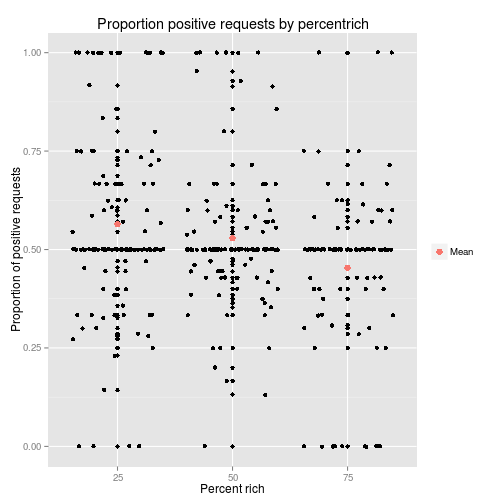
\includegraphics[width=.5\textwidth]{propposbypcrichdots.png}
\caption{Proportion of positive requests appear to cluster at values 0, 0.5, and 1. The observed differences between means may be driven by participants choosing between a small number of distinct request strategies.}
\label{propposdots}
\end{figure}

This clustering of request proportions motivates a categorization of responses by request strategy, `Prefers positive', `Even' and `Prefers negative'. An `Even' request strategy was defined as a proportion of positive requests falling between 0.45 and 0.55, with `Prefers positive' and `Prefers negative' responses falling above and below these values (Figure~\ref{sidebysidebar3}).

\begin{figure}[htb]
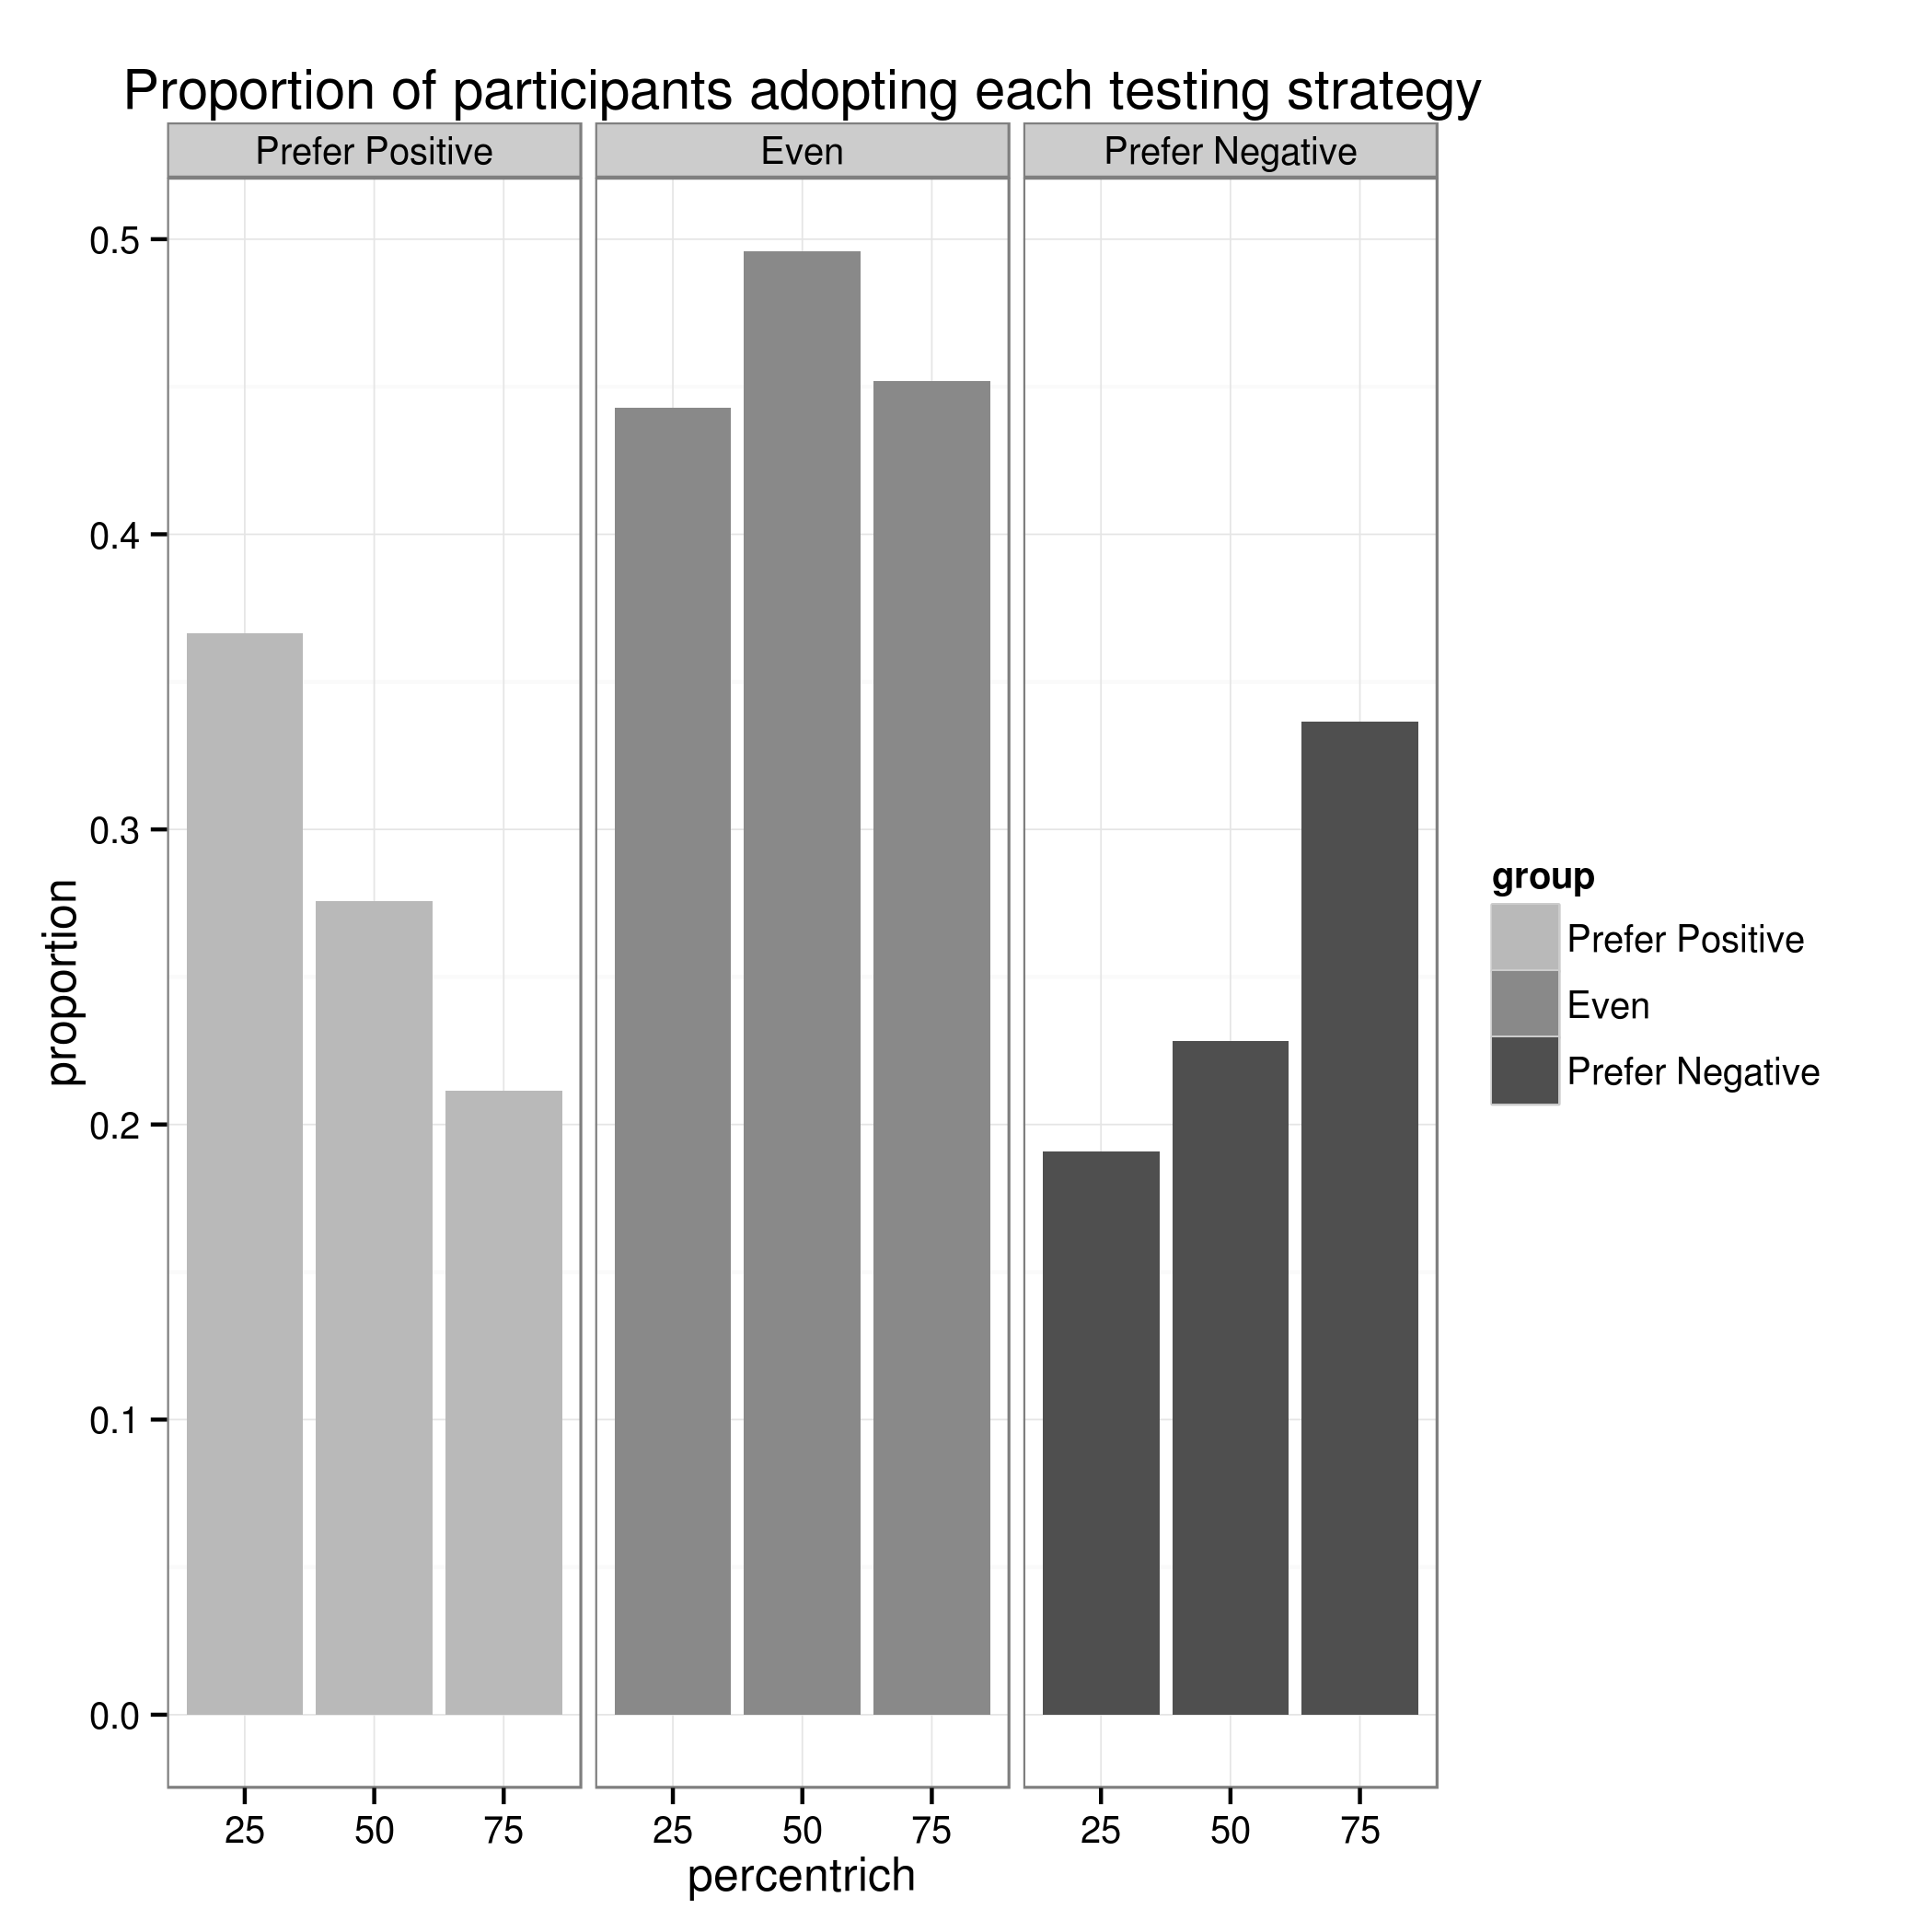
\includegraphics[width=.5\textwidth]{sidebysidebar3.png}
\caption{Proportion of participants using each testing strategy in the three conditions. Requesting equal amounts of information from both possible categorizations is always popular, however when population proportions are unequal, more people switch to preferring information about the minority group. This preference is somewhat asymmetrical, with people more readily switching to preferring positive requests}
\label{sidebysidebar3}
\end{figure}

All strategies were followed by some participants in all conditions, and the `Even' request strategy balancing positive and negative requests was always the most popular, never lower than 44\% of participants. The population percentage of `rich' plankton did impact on the attractiveness of each testing strategy: the proportion of people preferring positive tests fell from 37\% in the 25\% rich condition to 21\% in the 75\% rich condition, while the proportion of people preferring negative tests rose from 19\% to 33\%, indicating a preference for whichever type of test corresponded to the minority classification in the whole population. When the population was evenly split, the `Even' testing strategy was more popular than otherwise at 50\% of all participants, and a preference for positive tests was more common that a preference for negative tests, at 27\% and 23\% of participants respectively.

%What limitations/caveats/assumptions needed?
\section{Discussion}
%Conclusions
-Results show support for a sparsity effect consistent with battleships, \cite{navarro2011sparsecat}: effect of information sensitivity\\
-Results replicate a positivity/framing effect, it matters which side is `rich' \\
-Clustering at special values 0, .5, 1 in all conditions suggests a kind of heuristic approach. `context sensitive heuristics' (?) Not really a clean 100\% reliance on information value, anyway.\\

%Limitations
-Lots of drop-out, high exclusion rate. Suspicious?\\
-Visual box-sizes for grouping plankton, undermines claim of abstract hypothesis space?\\
-How critical is being able to see all possible plankton examples? Knowledge of limits of variation critical for sparsity manipulation? (Rarely available in real life...?)\\

%Further questions....
-How fine-grained are these judgements? Could a different design get smoother response variation with more smoothly varying information value, or (more) strategy-clusters in different places? (ie, battleships... so, yes?). Note everything here is discrete: features are discrete, selenoid status is binary, request type also binary, possibly this artificially encourages the clustering seen here? Testable: what if there are three categories, and three label-request buttons?\\
-Positivity bias attenuated in higher scoring group? (No relevant results reported in this draft). positivity bais possibly a fallback strategy, indicator of not understanding? Consistent with `naturalistic Wason improves performance' (others...?)\\


\section{Acknowledgements}

This research was supported by... 

\renewcommand{\bibliographytypesize}{\footnotesize}
\bibliographystyle{apacite}

\setlength{\bibleftmargin}{.125in}
\setlength{\bibindent}{-\bibleftmargin}


\bibliography{plankton.bib}


\end{document}